\section{Toolkit Overview}
In this section, we first introduce the design decisions and the overview of the toolkits. Then we present the user interface and the major functions.

The toolkit is designed and implemented as a web application, since it is easiest for crowd workers to visit.

The users of our visualization toolkit include {\em annotation gatherers} and {\em crowd-source workers}. In general, annotation gatherers (NLP experts and well-trained programmers) use our toolkit to collect training data from crowd-source workers for their NLP systems. We believe annotation gatherers know their NLP problems better than anyone else, so we leave them to implement a html page to display their problem. The html page would call the APIs to pass data (\eg\ objects to cluster) to the toolkits. The core component then is to visualize the problem, as well as allowing workers to interact with the objects. Our toolkit keeps the task-visualization transparent to maximize the flexibility of our toolkit. Figure~\ref{fig:workflow} shows the workflow of our toolkit.

\begin{figure}
\centering
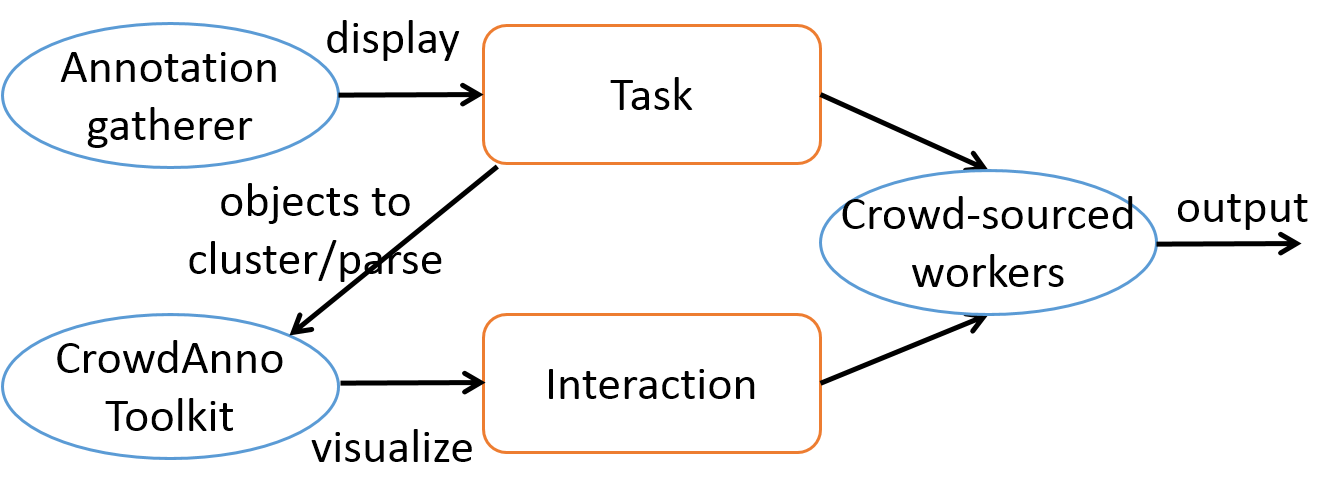
\includegraphics[width=3.1in]{figs/workflow.png}
\caption{Workflow of the toolkit: annotation gatherers generate the html pages to display the task; our toolkit take the html pages as the input and visualize the interactions; crowd-sourced workers see the integrated interface and generate the outputs. }
\label{fig:workflow}
\end{figure}

We use co-reference as the running example for clustering visualization. Figure~\ref{fig:interface1.png} shows the user interface. The left sides displays the NLP task. One simple way to display the co-reference task, as shown in the figure, is to highlight the mentions and to give them unique IDs. The right side of the interface is for the interaction purpose, where workers generate the clusters interactively. They can We will introduce the operators in details in Section 4.
\begin{figure*}
\centering
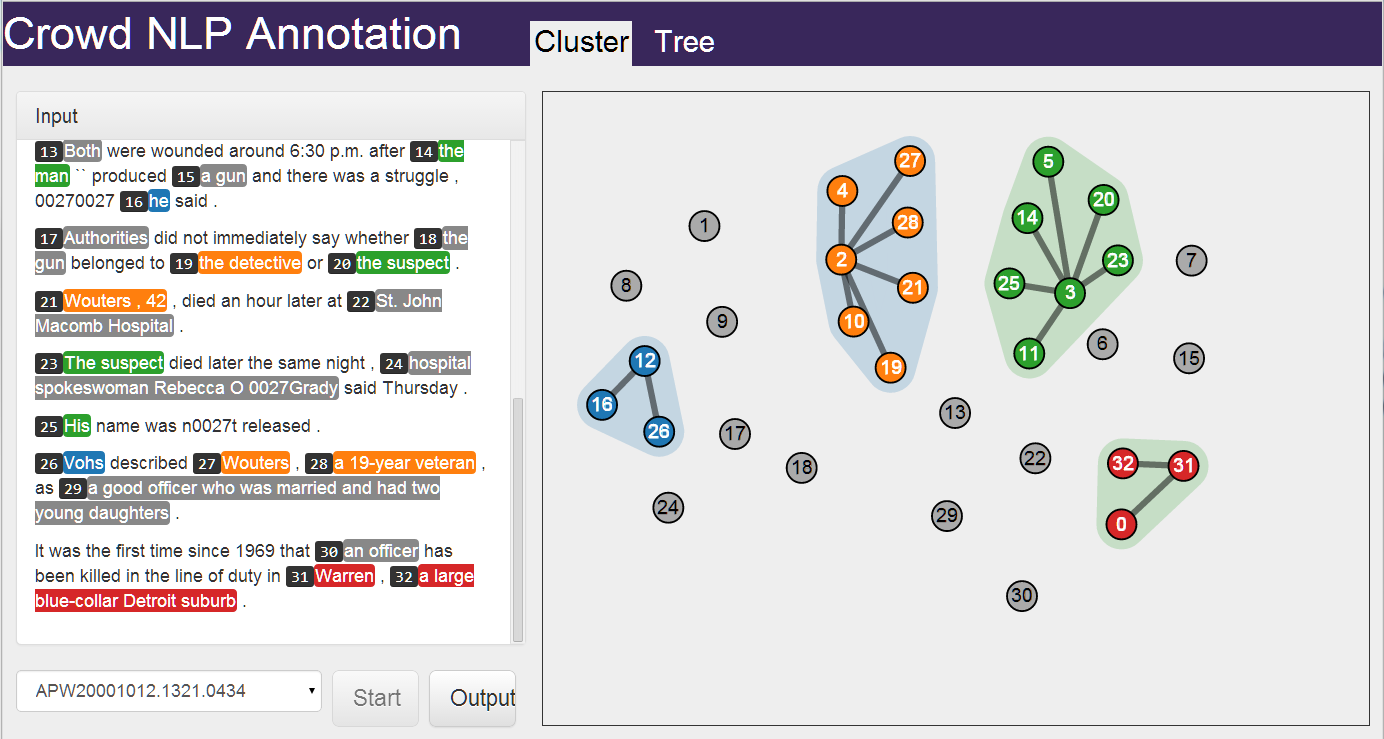
\includegraphics[width=6.1in]{figs/interface1_v2.png}
\caption{Interface of clustering: the left side displays the NLP task, which takes the input from annotator gatherer; the right side is the interaction area, where workers}
\label{fig:interface1.png}
\end{figure*}

We use syntactic parsing as the running example to show how our toolkit can build a parsed tree. To save the space, we only shows the trees before and after editing in the interaction area for sentence {\em ``There is no asbestos in our products now."}. Initially, workers see a ``flat" tree with sentence tokens as the leaf nodes. They can merge nodes, insert and delete branch nodes with some intuitive operators. Note that a valid tree should not change the order of the leaf nodes. We propose an innovative {\em line-intersect} operator to guarantee the validity. To our best knowledge, we are the first to propose this visualization operator on tree structure. We would introduce them in Section 5.

\begin{figure}
\centering
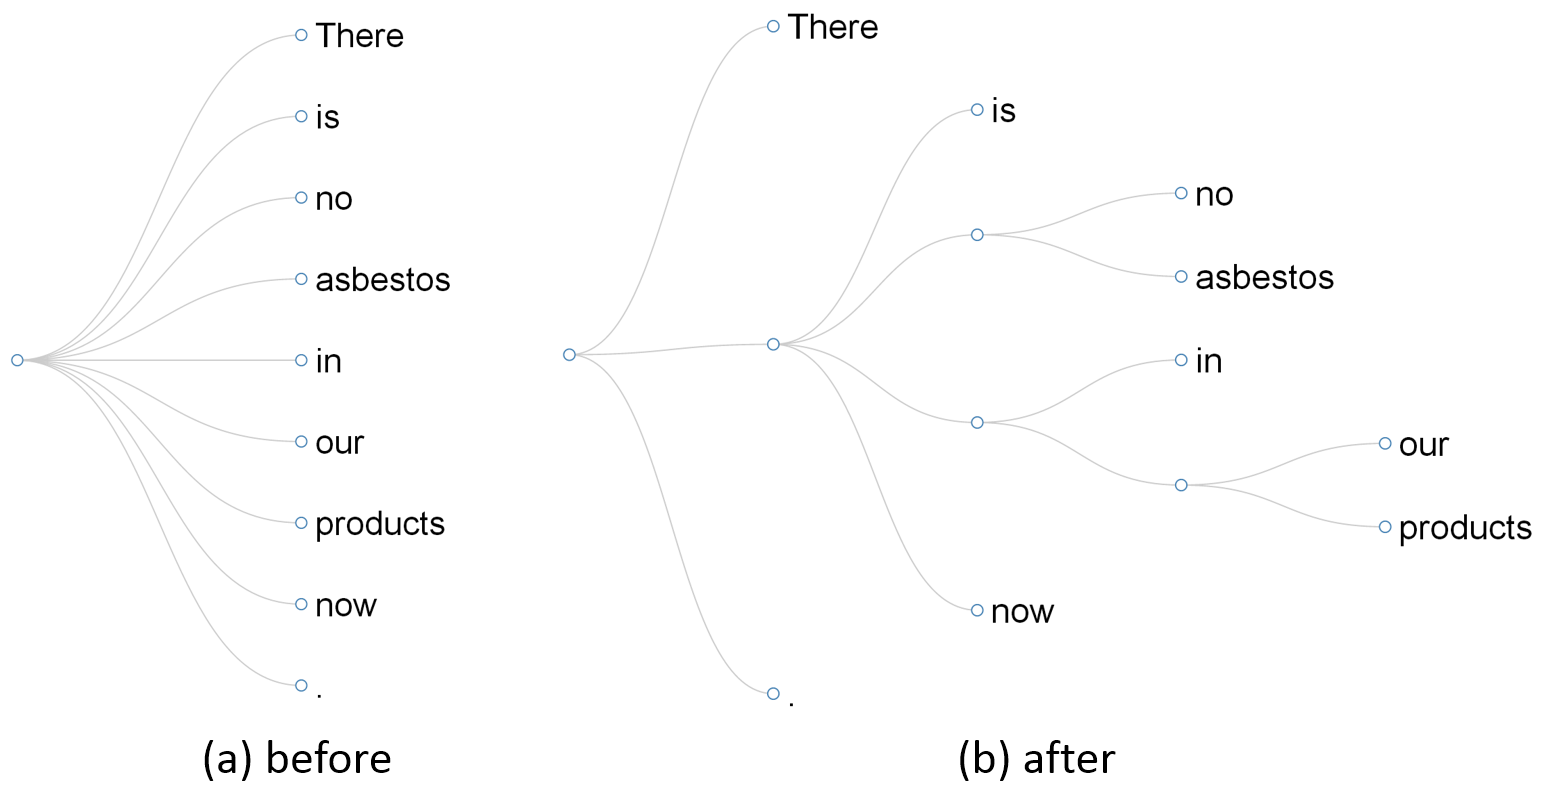
\includegraphics[width=3in]{figs/overview_tree_editing.png}
\caption{The before and after trees in the user interface when parsing the sentence {``There is no asbestos in our products now."}}
\label{fig:interface2.png}
\end{figure}

